\documentclass[dvips, lscape]{foils}
%\documentclass[dvips, french]{slides}
\textwidth 18.5cm
\textheight 25cm 
\topmargin -1cm 
\oddsidemargin  -1cm 
\evensidemargin  -1cm

% Maths
\usepackage{amsfonts, amsmath, amssymb, url}
\usepackage{/Latex/astats}

\newcommand{\coefbin}[2]{\left( 
    \begin{array}{c} #1 \\ #2 \end{array} 
  \right)}
\newcommand{\bbullet}{\bullet\bullet}
\newcommand{\bbbullet}{\bbullet\bullet}
\newcommand{\bbbbullet}{\bbbullet\bullet}
\newcommand{\Acal}{\mathcal{A}}
\newcommand{\Bcal}{\mathcal{B}}
\newcommand{\Ccal}{\mathcal{C}}
\newcommand{\Dcal}{\mathcal{D}}
\newcommand{\Ecal}{\mathcal{E}}
\newcommand{\Gcal}{\mathcal{G}}
\newcommand{\Mcal}{\mathcal{M}}
\newcommand{\Ncal}{\mathcal{N}}
\newcommand{\Ocal}{\mathcal{O}}
\newcommand{\Pcal}{\mathcal{P}}
\newcommand{\Qcal}{\mathcal{Q}}
\newcommand{\Rcal}{\mathcal{R}}
\newcommand{\Hcal}{\mathcal{H}}
\newcommand{\Jcal}{\mathcal{J}}
\newcommand{\Lcal}{\mathcal{L}}
\newcommand{\Tcal}{\mathcal{T}}
\newcommand{\Ucal}{\mathcal{U}}
\newcommand{\Xcal}{\mathcal{X}}
\newcommand{\Zcal}{\mathcal{Z}}
\newcommand{\etabar}{\overline{\eta}}
\newcommand{\pibar}{\overline{\pi}}
\newcommand{\alphabf}{\mbox{\mathversion{bold}{$\alpha$}}}
\newcommand{\betabf}{\mbox{\mathversion{bold}{$\beta$}}}
\newcommand{\gammabf}{\mbox{\mathversion{bold}{$\gamma$}}}
\newcommand{\mubf}{\mbox{\mathversion{bold}{$\mu$}}}
\newcommand{\Pibf}{\mbox{\mathversion{bold}{$\Pi$}}}
\newcommand{\psibf}{\mbox{\mathversion{bold}{$\psi$}}}
\newcommand{\Sigmabf}{\mbox{\mathversion{bold}{$\Sigma$}}}
\newcommand{\taubf}{\mbox{\mathversion{bold}{$\tau$}}}
\newcommand{\thetabf}{\mbox{\mathversion{bold}{$\theta$}}}
\newcommand{\Abf}{{\bf A}}
\newcommand{\Ebf}{{\bf E}}
\newcommand{\Hbf}{{\bf H}}
\newcommand{\Ibf}{{\bf I}}
\newcommand{\Obf}{{\bf 0}}
\newcommand{\Sbf}{{\bf S}}
\newcommand{\mbf}{{\bf m}}
\newcommand{\ubf}{{\bf u}}
\newcommand{\vbf}{{\bf v}}
\newcommand{\wbf}{{\bf w}}
\newcommand{\xbf}{{\bf x}}
\newcommand{\Xbf}{{\bf X}}
\newcommand{\Esp}{{\mathbb E}}
\newcommand{\Corr}{{\mathbb C}\mbox{orr}}
\newcommand{\Nm}{N(\mbf)}
\newcommand{\mum}{\mu(\mbf)}
\newcommand{\obs}{\text{obs}}
\newcommand{\ERMG}{\text{EMRG}}
\newcommand{\Ibb}{{\mathbb I}}
\newcommand{\Omegas}{\underset{s}{\Omega}}
\newcommand{\Var}{{\mathbb V}}
\newcommand{\Rbb}{\mathbb{R}}
\newcommand{\Vsf}{\mathsf{V}}
\newcommand{\Starsf}{\mathsf{*}}

% Couleur et graphiques
\usepackage{color}
\usepackage{graphics}
\usepackage{epsfig} 
\usepackage{pstcol}

% Texte
\usepackage{lscape}
\usepackage{../../../../Latex/fancyheadings, rotating, enumerate}
%\usepackage[french]{babel}
\usepackage[latin1]{inputenc}
%\definecolor{darkgreen}{cmyk}{0.5, 0, 0.5, 0.5}
%\definecolor{green}{cmyk}{0.5, 0, 0.5, 0.5}
\definecolor{orange}{cmyk}{0, 0.6, 0.8, 0}
\definecolor{jaune}{cmyk}{0, 0.5, 0.5, 0}
\newcommand{\textblue}[1]{\textcolor{blue}{#1}}
\newcommand{\textred}[1]{\textcolor{red}{#1}}
\newcommand{\textgreen}[1]{\textcolor{green}{ #1}}
\newcommand{\textlightgreen}[1]{\textcolor{green}{#1}}
%\newcommand{\textgreen}[1]{\textcolor{darkgreen}{#1}}
\newcommand{\textorange}[1]{\textcolor{orange}{#1}}
\newcommand{\textyellow}[1]{\textcolor{yellow}{#1}}
\newcommand{\emphase}[1]{\textblue{\sl #1}}
\newcommand{\refer}[1]{\textgreen{\sl \cite{#1}}}

% Listes
\newcommand{\itemv}{\item \vspace{-0.5cm}}

% Sections
%\newcommand{\chapter}[1]{\centerline{\LARGE \textblue{#1}}}
% \newcommand{\section}[1]{\centerline{\Large \textblue{#1}}}
% \newcommand{\subsection}[1]{\noindent{\Large \textblue{#1}}}
% \newcommand{\subsubsection}[1]{\noindent{\large \textblue{#1}}}
% \newcommand{\paragraph}[1]{\noindent {\textblue{#1}}}
% Sectionsred
\newcommand{\chapter}[1]{
  \addtocounter{chapter}{1}
  \setcounter{section}{0}
  \setcounter{subsection}{0}
  {\centerline{\LARGE \textblue{\arabic{chapter} - #1}}}
%  {\centerline{\LARGE \textblue{#1}}}
  }
\newcommand{\section}[1]{
  \addtocounter{section}{1}
  \setcounter{subsection}{0}
  {\noindent {\Large \textblue{\arabic{chapter}.\arabic{section} - #1}}}
%  {\noindent {\Large \textblue{#1}}}
  }
\newcommand{\subsection}[1]{
  \addtocounter{subsection}{1}
%   {\noindent{\large
%       \textblue{\arabic{chapter}.\arabic{section}.\arabic{subsection}
%         - #1}}}
  {\noindent{\large \textblue{#1}}}
  }
\newcommand{\paragraph}[1]{\noindent{\textblue{#1}}}

%%%%%%%%%%%%%%%%%%%%%%%%%%%%%%%%%%%%%%%%%%%%%%%%%%%%%%%%%%%%%%%%%%%%%%
%%%%%%%%%%%%%%%%%%%%%%%%%%%%%%%%%%%%%%%%%%%%%%%%%%%%%%%%%%%%%%%%%%%%%%
%%%%%%%%%%%%%%%%%%%%%%%%%%%%%%%%%%%%%%%%%%%%%%%%%%%%%%%%%%%%%%%%%%%%%%
%%%%%%%%%%%%%%%%%%%%%%%%%%%%%%%%%%%%%%%%%%%%%%%%%%%%%%%%%%%%%%%%%%%%%%
\begin{document}
%%%%%%%%%%%%%%%%%%%%%%%%%%%%%%%%%%%%%%%%%%%%%%%%%%%%%%%%%%%%%%%%%%%%%%
%%%%%%%%%%%%%%%%%%%%%%%%%%%%%%%%%%%%%%%%%%%%%%%%%%%%%%%%%%%%%%%%%%%%%%
%%%%%%%%%%%%%%%%%%%%%%%%%%%%%%%%%%%%%%%%%%%%%%%%%%%%%%%%%%%%%%%%%%%%%%
%%%%%%%%%%%%%%%%%%%%%%%%%%%%%%%%%%%%%%%%%%%%%%%%%%%%%%%%%%%%%%%%%%%%%%
\landscape
\newcounter{chapter}
\newcounter{section}
\newcounter{subsection}
\setcounter{chapter}{0}
\headrulewidth 0pt 
\pagestyle{fancy} 
\cfoot{}
\rfoot{
%   \begin{rotate}{90}{
%       \hspace{1cm} \tiny S. Robin: Assessing the exceptionality of
%       network motifs  
%       }\end{rotate}
}
\rhead{\begin{rotate}{90}{
      \hspace{-.5cm} \tiny \thepage
      }\end{rotate}}

%%%%%%%%%%%%%%%%%%%%%%%%%%%%%%%%%%%%%%%%%%%%%%%%%%%%%%%%%%%%%%%%%%%%%%
%%%%%%%%%%%%%%%%%%%%%%%%%%%%%%%%%%%%%%%%%%%%%%%%%%%%%%%%%%%%%%%%%%%%%%
\begin{center}
  \textblue{\LARGE Assessing the exceptionality of network motifs}
  
  \vspace{1cm}
  \textblue{\large S. Robin} \\
  ~\\
  {\tt robin@agroparistech.fr} \\
  ~\\
  {\large Joint work with \textblue{J.-J. Daudin, M. Koskas, F. Picard
      and S. Schbath}}
  ~\\ ~\\
\end{center}

\noindent UMR AgroParisTech / INRA, Paris, Math�matique et Informatique Appliqu�es~: \\
\centerline{\url{www.agroparistech.fr/mia/}}

\noindent {Statistics for Systems Biology (SSB) group:} \\
\centerline{\url{genome.jouy.inra.fr/ssb/}} \\


\paragraph{Research report:} \\
\centerline{\url{genome.jouy.inra.fr/ssb/preprint/SSB-RR-1.netmotifs.pdf}}
+ 
\newblock {\em J. Comp. Biol.}  \newblock (2008).  \newblock {\bf
  15}~{\bf (1)} 1--20.
%\refer{PDK08}

%%%%%%%%%%%%%%%%%%%%%%%%%%%%%%%%%%%%%%%%%%%%%%%%%%%%%%%%%%%%%%%%%%%%%
%%%%%%%%%%%%%%%%%%%%%%%%%%%%%%%%%%%%%%%%%%%%%%%%%%%%%%%%%%%%%%%%%%%%%
\newpage
\chapter{Network motifs}
%%%%%%%%%%%%%%%%%%%%%%%%%%%%%%%%%%%%%%%%%%%%%%%%%%%%%%%%%%%%%%%%%%%%%
%%%%%%%%%%%%%%%%%%%%%%%%%%%%%%%%%%%%%%%%%%%%%%%%%%%%%%%%%%%%%%%%%%%%%

%%%%%%%%%%%%%%%%%%%%%%%%%%%%%%%%%%%%%%%%%%%%%%%%%%%%%%%%%%%%%%%%%%%%%
\bigskip
\section{Analysing biological interaction networks}
%%%%%%%%%%%%%%%%%%%%%%%%%%%%%%%%%%%%%%%%%%%%%%%%%%%%%%%%%%%%%%%%%%%%%

%%%%%%%%%%%%%%%%%%%%%%%%%%%%%%%%%%%%%%%%%%%%%%%%%%%%%%%%%%%%%%%%%%%%%
\subsection{Interaction networks}

\paragraph{Many scientific fields:} sociology, physics, "internet",
  biology.

\paragraph{Data:} 
\begin{itemize}
\item \vspace{-0.5cm} interactions between $n$ elements (nodes), 
\item \vspace{-0.5cm} $n^2$ possible interactions (edges).
\end{itemize}

\paragraph{Topology of the network:}
\begin{itemize}
\item \vspace{-0.5cm} describes the way genes/proteins interact,
\item \vspace{-0.5cm} structural properties (degrees, diameter,
  clustering coefficient), 
\item \vspace{-0.5cm} \emphase{recurrent patterns (motifs)}.
\end{itemize}

% \vspace{-10mm}
% \begin{center}
% \includegraphics[angle=90,height=6cm,width=6cm]{./figures/barabasi6.ps}\\
% \begin{tiny} \qquad\qquad From Barabasi et al.(2004) \end{tiny}
% \end{center}

%%%%%%%%%%%%%%%%%%%%%%%%%%%%%%%%%%%%%%%%%%%%%%%%%%%%%%%%%%%%%%%%%%%%%
\newpage
\section{Over-represented motifs}
%%%%%%%%%%%%%%%%%%%%%%%%%%%%%%%%%%%%%%%%%%%%%%%%%%%%%%%%%%%%%%%%%%%%%

\paragraph{Patterns of interconnection, motifs:}
One way to understand how complex network behave is to break them down
complex networks into \emphase{functional modules} or basic building
blocks. \refer{SMM02}

\bigskip
\hspace{-2.2cm}
\begin{tabular}{lcc}
  \begin{tabular}{p{15cm}}
    \paragraph{Transcription regulatory networks:} 
    motifs may perform specific regulatory functions
    (e.g. feed-forward loop, bi-fan).
  \end{tabular}
  &
  \begin{tabular}{c}
    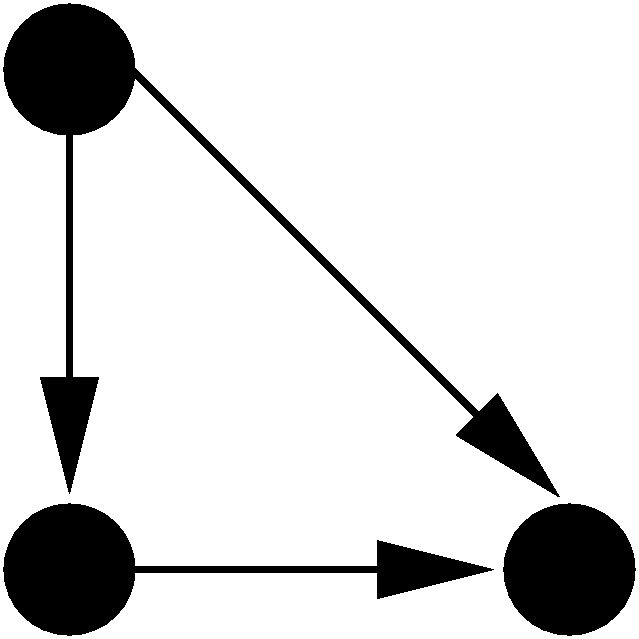
\epsfig{file=../Figures/feedforwardloop.eps, clip=}
  \end{tabular}
  &
  \begin{tabular}{c}
    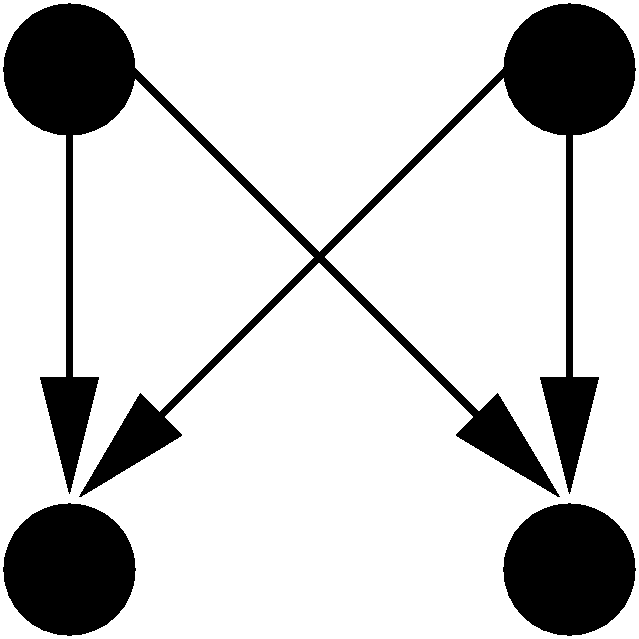
\epsfig{file=../Figures/bifan.eps, clip=}
  \end{tabular}
\end{tabular}

\bigskip
\paragraph{Focus on exceptional motif}  
$=$ motifs appearing more \emphase{frequently than expected}.
\refer{MSI02},  \refer{SMM02}, \refer{ZKW05}

\bigskip
\paragraph{Interpretation:} 
Such motifs are thought to reflect \emphase{functional units} which
combine to
regulate the cellular behavior as a whole. \\
$\Rightarrow$ Mathematical analysis of their dynamics are required.
\refer{MaA03}, \refer{PIL05}

%%%%%%%%%%%%%%%%%%%%%%%%%%%%%%%%%%%%%%%%%%%%%%%%%%%%%%%%%%%%%%%%%%%%%
\newpage
\section{Assessing the exceptionality of a motif}

\subsection{We have to}
\begin{enumerate}
\item \emphase{Count} the observed number of occurrences
  $N_{\obs}(\mbf)$ of a given motif $\mbf$. \\
  (Out of our scope?)
\item Choose an appropriate \emphase{random graph model}.
\item Derive the \emphase{distribution} of the count $\Nm$.
\item \emphase{Assess} its significance with the $p$-value
  $$
  \Pr\{\Nm \geq N_{\obs}(\mbf)\}
  $$
\end{enumerate}

%%%%%%%%%%%%%%%%%%%%%%%%%%%%%%%%%%%%%%%%%%%%%%%%%%%%%%%%%%%%%%%%%%%%%
\newpage
\subsection{Motif count distribution: State of the art}

\paragraph{Asymptotic approximations (Gaussian, Poisson, Compound
  Poisson)}. Many papers about the asymptotic distribution of the
  count $\Nm$. 
\begin{itemize}
\item Most of the times, only \emphase{simple models} (Erd�s-R�nyi) or
  \emphase{simple motifs} (triangle) are considered.
\item The underlying hypotheses are very \emphase{restrictive} and
  depend on the structure of the motif itself.
\end{itemize}

\bigskip\bigskip
\paragraph{Standard approach in biological applications.}
When analysing motifs in biological networks, the most common strategy
is based on simulations, empiricalmoments and/or empirical
distribution (\refer{SMM02}).

% \bigskip
% \paragraph{Standard approach in biological applications.}
% When analysing motifs in biological networks, the most common strategy
% is based on simulations using the following scheme (\refer{SMM02}):
% \begin{enumerate}
% \item \vspace{-0.5cm} generate a \emphase{large number} of random
%   networks (e.g. by edge swapping),
% \item \vspace{-0.5cm} get the \emphase{empirical distribution} of the count,
% \item \vspace{-0.5cm} calculate a $Z$ ($\Rightarrow$ Gaussian
%   approximation?) or an empirical $p$-value.
% \end{enumerate}

%%%%%%%%%%%%%%%%%%%%%%%%%%%%%%%%%%%%%%%%%%%%%%%%%%%%%%%%%%%%%%%%%%%%%%%%
\newpage
\noindent
\begin{tabular}{cc}
  \begin{tabular}{p{15cm}}
    \subsection{\refer{SMM02}:} \\
    \\
    Search for \textblue{over-represented motifs} in {\sl E. coli}
    transcriptional network. \\
    \\
    \paragraph{Strategy.} 
    \begin{enumerate}
    \item Count the number of occurrences $N_{\obs}(\mbf)$; 
    \item Resample a \textblue{large number of random networks}
      similar to {\sl E.coli}'s one (e.g. same degree for each gene);
    \item Estimate $\Esp \Nm$ and $\Var \Nm$;
    \item Calculate a $Z$-score: 
      $Z = (N_{\obs}(\mbf) - \Esp \Nm)/ \sqrt{\Var \Nm}$;
    \item \textblue{Derive a $p$-value} implicitly based on a Gaussian approximation.
    \end{enumerate}
  \end{tabular}
  &
  \begin{tabular}{c}
    \epsfig{file=../FIGURES/RegulationMotifs.ps, bbllx=82, bblly=89, bburx=289, bbury=600, clip=}
  \end{tabular}
\end{tabular}

%%%%%%%%%%%%%%%%%%%%%%%%%%%%%%%%%%%%%%%%%%%%%%%%%%%%%%%%%%%%%%%%%%%%%
\newpage
\section{Our contribution}
%%%%%%%%%%%%%%%%%%%%%%%%%%%%%%%%%%%%%%%%%%%%%%%%%%%%%%%%%%%%%%%%%%%%%

\begin{itemize}
\item We provide \emphase{analytical expressions of the mean and the
  variance} of the count in a \emphase{wide class of random graph
    models}.
\item We propose an \emphase{approximate distribution} of the count
  and assess its quality via simulations.
\item We propose a \emphase{new random graph model} adapted for
  biological networks.
\end{itemize}

\bigskip\bigskip
%%%%%%%%%%%%%%%%%%%%%%%%%%%%%%%%%%%%%%%%%%%%%%%%%%%%%%%%%%%%%%%%%%%%%
\subsection{Orientation of the graph} 

Biological network may be oriented (regulation) or non oriented
(protein-protein interaction, PPI).

All results presented here are for non-oriented network; They can all
be generalised to oriented ones.

%%%%%%%%%%%%%%%%%%%%%%%%%%%%%%%%%%%%%%%%%%%%%%%%%%%%%%%%%%%%%%%%%%%%%
%%%%%%%%%%%%%%%%%%%%%%%%%%%%%%%%%%%%%%%%%%%%%%%%%%%%%%%%%%%%%%%%%%%%%
\newpage
\chapter{Sequence motifs}
%%%%%%%%%%%%%%%%%%%%%%%%%%%%%%%%%%%%%%%%%%%%%%%%%%%%%%%%%%%%%%%%%%%%%
%%%%%%%%%%%%%%%%%%%%%%%%%%%%%%%%%%%%%%%%%%%%%%%%%%%%%%%%%%%%%%%%%%%%%

\bigskip\bigskip
\centerline{\emphase{Back in time...}}

%%%%%%%%%%%%%%%%%%%%%%%%%%%%%%%%%%%%%%%%%%%%%%%%%%%%%%%%%%%%%%%%%%%%%
\bigskip\bigskip
\subsection{General problem}

Motif statistics aim at detecting functional motif in DNA or protein
sequences, based on their frequencies.

\bigskip\bigskip
\paragraph{Typical questions.}
\begin{itemize}
\item The \emphase{motif {\tt gctggtgg}} occurs more than 600
  times in the genome of {\sl E. Coli} that is 4.8 Mb long.
  \emphase{Is it much?}
\item Palindromes (i.e. self-complementary motifs) seem to be avoided
  in the same genome. Is this \emphase{under-representation
  significant}? 
\end{itemize}
\refer{RRS05}

%%%%%%%%%%%%%%%%%%%%%%%%%%%%%%%%%%%%%%%%%%%%%%%%%%%%%%%%%%%%%%%%%%%%%
\newpage
\section{Motifs occurrences}
%%%%%%%%%%%%%%%%%%%%%%%%%%%%%%%%%%%%%%%%%%%%%%%%%%%%%%%%%%%%%%%%%%%%%

\bigskip
\paragraph{Sequence.} $\Xbf$ is a random sequence with length
$n$ over an alphabet $\Acal$ (e.g. $\Acal = \{{\tt a, c, g, t}\})$:
$$
\Xbf = (X_1, X_2, \dots, X_n), \qquad X_i \in \Acal.
$$
\paragraph{Motif.} A motif (word) $\wbf$ is a (short) sequence of
letter over the same alphabet:
$$
\wbf = (w_1, w_2, \dots, w_k), \qquad w_u \in \Acal.
$$
\paragraph{Motif occurrence.} $\wbf$ is said to occur (i.e. to end)
\emphase{at position $i$} if  
$$
(X_{i-k+1}, \dots, X_i) = (w_1, \dots, w_k).
$$
\paragraph{Occurrence indicator:}
$$
Y_i(\wbf) = \Ibb\{(X_{i-k+1}, \dots, X_i) = (w_1, \dots, w_k)\}, 
\qquad k \leq i \leq n.
$$
\paragraph{Count.} The number of occurrences of $\wbf$ in $\Xbf$ is
$\displaystyle{\emphase{
N(\wbf) = \sum_{i=k}^n Y_i(\wbf).
}}$

%%%%%%%%%%%%%%%%%%%%%%%%%%%%%%%%%%%%%%%%%%%%%%%%%%%%%%%%%%%%%%%%%%%%%
\newpage
\section{Counts for Markov models}
%%%%%%%%%%%%%%%%%%%%%%%%%%%%%%%%%%%%%%%%%%%%%%%%%%%%%%%%%%%%%%%%%%%%%

\bigskip
\paragraph{Markov model.}
$\Xbf$ is supposed to be a Markov chain of order $m$ (M$m$) with
transition $\pi$:
$$
\Pr\{X_i = b | \Xbf_1^i\} 
= \Pr\{X_i = b | X_{i_m} = a_1, \dots X_{i_1} = a_m\}
= \pi(a_1, \dots a_m ; b).
$$

\bigskip
\paragraph{Choosing the right model.} The transition $\pi$ is
estimated by
$$
\widehat{\pi}(a_1, \dots a_m ; b) = N(a_1, \dots, a_m, b) / N(a_1,
\dots, a_m)
$$
so the M$m$ model \emphase{accounts for the counts of all words of
  length $m+1$}.

\bigskip
\paragraph{Maximal model.} To study the significance of the count
$N(\wbf)$, the maximal model is 
$$
\emphase{\text{M}(k-2)}.
$$
All models with $m \geq k-1$ will \emphase{exactly fit to $N(\wbf)$}.

%%%%%%%%%%%%%%%%%%%%%%%%%%%%%%%%%%%%%%%%%%%%%%%%%%%%%%%%%%%%%%%%%%%%%
\newpage
\section{Moments of the count}
%%%%%%%%%%%%%%%%%%%%%%%%%%%%%%%%%%%%%%%%%%%%%%%%%%%%%%%%%%%%%%%%%%%%%

\bigskip
\paragraph{Expectation of the count.} The expected count is
$$
\Esp N(\wbf) = \sum_i \Esp Y_i(\wbf) = (n-k+1) \mu(\wbf)
$$
where $\mu$ stands for the \emphase{stationary distribution} of $\pi$:
$$
\mu(\wbf) = \mu(w_1, \dots, w_{k-1}) \pi(w_1, \dots, w_{k-1}; w_k).
$$

\bigskip
\paragraph{Variance of the count.} The get the variance, we have to
calculate
$$
\Esp N^2(\wbf) 
= \sum_i \Esp Y_i 
+ \underset{\text{\normalsize \emphase{overlapping
      occurrences}}}{\underbrace{\sum_i \sum_{j: |i-j| < k} \Esp (Y_i
    Y_j)}}     
+ \sum_i \sum_{j: |i-j| \geq k} \Esp (Y_i Y_j)
$$
{\tt atatat} can overlap, whereas {\tt gatcat} can not...

%%%%%%%%%%%%%%%%%%%%%%%%%%%%%%%%%%%%%%%%%%%%%%%%%%%%%%%%%%%%%%%%%%%%%
\newpage
\section{Distribution of the count}
%%%%%%%%%%%%%%%%%%%%%%%%%%%%%%%%%%%%%%%%%%%%%%%%%%%%%%%%%%%%%%%%%%%%%

\bigskip
\paragraph{Exact distribution.} The generating function of $N(\wbf)$
(and associated quantities) can be derived, but its Taylor expansion
is \emphase{very demanding for large sequence}.

\bigskip
\paragraph{Approximate distribution.}
\begin{itemize}
\itemv The limit distribution for frequent word ($\Esp N = \Ocal(n)$)
  is \emphase{Gaussian}.
\itemv \emphase{Compound Poisson} is the limit distribution for rare
  words ($\Esp N = \Ocal(\log n)$).
\end{itemize}
\paragraph{Compound Poisson heuristic.} \\
\centerline{
  \psfig{file = ../FIGURES/FigPoissonComp.ps,
    height=3.9cm, width=25cm, bbllx=80 , bblly=260 , bburx=525 ,
    bbury=330, clip=}
}
Occurrences are \emphase{gathered in $C$ clumps} with respective sizes $(K_1,
  \dots, K_C)$: \\
$$
C \sim \Pcal\{[1-a(\wbf)]\mu(\wbf)\}, 
\qquad \{K_i\} \text{ i.i.d. } \sim \Gcal[1-a(\wbf)]
\qquad N = \sum_{c=1}^C K_c
$$
where $a(\wbf)$ stands for the \emphase{overlapping probability} if $\wbf$.

%%%%%%%%%%%%%%%%%%%%%%%%%%%%%%%%%%%%%%%%%%%%%%%%%%%%%%%%%%%%%%%%%%%%%
%%%%%%%%%%%%%%%%%%%%%%%%%%%%%%%%%%%%%%%%%%%%%%%%%%%%%%%%%%%%%%%%%%%%%
\newpage
\chapter{Motif Occurrences and Count}
%%%%%%%%%%%%%%%%%%%%%%%%%%%%%%%%%%%%%%%%%%%%%%%%%%%%%%%%%%%%%%%%%%%%%
%%%%%%%%%%%%%%%%%%%%%%%%%%%%%%%%%%%%%%%%%%%%%%%%%%%%%%%%%%%%%%%%%%%%%

%%%%%%%%%%%%%%%%%%%%%%%%%%%%%%%%%%%%%%%%%%%%%%%%%%%%%%%%%%%%%%%%%%%%%
\bigskip
\section{Motif and permutations}
%%%%%%%%%%%%%%%%%%%%%%%%%%%%%%%%%%%%%%%%%%%%%%%%%%%%%%%%%%%%%%%%%%%%%

\paragraph{Definition.}  A motif $\mbf$ of size $k$ is a connected
sub-graph with $k$ vertices characterised by its adjacency matrix
(also denoted by $\mbf$):
$$
m_{uv} = \Ibb\{u \sim v\}.
$$

\hspace{-2.2cm}
\begin{tabular}{cc}
  \begin{tabular}{p{10cm}}
    \paragraph{Permutations.} For a given motif $\mbf$, we need to
    consider the set $\Rcal(\mbf)$ of its permutations. \\
    \\
    For example, the $\mathsf{V}$ motif may occure in 3 ways at a
    \emphase{fixed} position $\alpha = (i,j,k)$: \\
    \\
  \end{tabular}
  &
  \begin{tabular}{ccc}
    $\mbf$ &  $\mbf^{\prime}$ & $\mbf^{\prime \prime}$ \\
    & & \\
    $\left[ \begin{array}{ccc} 
        0 & 1 & 1 \\ . & 0 & 0 \\ . & . & 0 
      \end{array} \right]$  &
    $\left[ \begin{array}{ccc} 
        0 & 1 & 0 \\ . & 0 & 1 \\ . & . & 0 
      \end{array} \right]$ &
    $\left[ \begin{array}{ccc} 
        0 & 0 & 1 \\ . & 0 & 1 \\ . & . & 0 
      \end{array} \right] $ \\
    &&
    \\
    \epsfig{file=../Figures/version2.eps} & 
    \epsfig{file=../Figures/version3.eps} & 
    \epsfig{file=../Figures/version1.eps} 
  \end{tabular}
\end{tabular}

%%%%%%%%%%%%%%%%%%%%%%%%%%%%%%%%%%%%%%%%%%%%%%%%%%%%%%%%%%%%%%%%%%%%%
\newpage
\section{Count}
%%%%%%%%%%%%%%%%%%%%%%%%%%%%%%%%%%%%%%%%%%%%%%%%%%%%%%%%%%%%%%%%%%%%%

\paragraph{Position.} A ($k$-)position $\alpha$ is a set of $k$
different nodes taken is ascending order:
$$
\alpha = (i_1, ... i_k), \qquad i_1 < i_2 < ... < i_k.
$$
A graph of size $n$ contains $\displaystyle{\binom{n}{k}}$ positions.

\paragraph{Occurrence.} $Y_{\alpha}(\mbf)$ is the \emphase{binary
  variable} indicating if $\mbf$ occurs at position $\alpha$:
$$
Y_{\alpha}(\mbf) 
= \Ibb\{\mbf \text{ occurs at } \alpha\}
=\prod_{1 \leq u < v \leq k} (X_{i_ui_v})^{m_{uv}}.
$$

\paragraph{Count.} The total number of occurrences of $\mbf$ in the
graph is the sum over \emphase{all positions} and \emphase{all
  permutations} of the binary variables $Y_{\alpha}(\mbf)$:
$$
N(\mbf) = \sum_{\alpha} \sum_{\mbf' \in \Rcal(\mbf)} Y_{\alpha}(\mbf').
$$

%%%%%%%%%%%%%%%%%%%%%%%%%%%%%%%%%%%%%%%%%%%%%%%%%%%%%%%%%%%%%%%%%%%%%
%%%%%%%%%%%%%%%%%%%%%%%%%%%%%%%%%%%%%%%%%%%%%%%%%%%%%%%%%%%%%%%%%%%%%
\newpage
\chapter{Random Graph Model}
%%%%%%%%%%%%%%%%%%%%%%%%%%%%%%%%%%%%%%%%%%%%%%%%%%%%%%%%%%%%%%%%%%%%%
%%%%%%%%%%%%%%%%%%%%%%%%%%%%%%%%%%%%%%%%%%%%%%%%%%%%%%%%%%%%%%%%%%%%%

%%%%%%%%%%%%%%%%%%%%%%%%%%%%%%%%%%%%%%%%%%%%%%%%%%%%%%%%%%%%%%%%%%%%%
\bigskip\bigskip
\section{Random graph model}
%%%%%%%%%%%%%%%%%%%%%%%%%%%%%%%%%%%%%%%%%%%%%%%%%%%%%%%%%%%%%%%%%%%%%

\paragraph{Notations.} We denote $i=1..n$ the (fixed) nodes and $X_{ij}$
the (random) edges:
$$
X_{ij} = \Ibb\{i \sim j\}.
$$
A random graph $G$ is completely characterised by $n$ and the
$X_{ij}$'s.

\bigskip\bigskip
\paragraph{Random graph model.} 
A random graph model is needed to derive de distribution of the count
$\Nm$. Such a model must specifies the \emphase{joint distribution of
  the $X_{ij}$'s}. 

The distribution of the degrees of the nodes is \emphase{not sufficient}.

%%%%%%%%%%%%%%%%%%%%%%%%%%%%%%%%%%%%%%%%%%%%%%%%%%%%%%%%%%%%%%%%%%%%%
\newpage
\section{Some examples}
%%%%%%%%%%%%%%%%%%%%%%%%%%%%%%%%%%%%%%%%%%%%%%%%%%%%%%%%%%%%%%%%%%%%%

%%%%%%%%%%%%%%%%%%%%%%%%%%%%%%%%%%%%%%%%%%%%%%%%%%%%%%%%%%%%%%%%%%%%%
\subsection{Erd�s-R�nyi}

The oldest and simplest model assumes the edges are independent and
exist with the same probability:
$$
\{X_{ij}\} \text{ i.i.d.}, \qquad X_{ij} \sim \Bcal(\pi).
$$
The degree $K_i = \sum_{j \neq i} X_{ij}$ has a binomial
(approximately Poisson) distribution.

%%%%%%%%%%%%%%%%%%%%%%%%%%%%%%%%%%%%%%%%%%%%%%%%%%%%%%%%%%%%%%%%%%%%%
\bigskip\bigskip
\subsection{Fitting the degree distribution}

The degree of the nodes is characteristic that one may like to
preserve. Denoting $\{k_1, .. k_n\}$ the degrees of the nodes is the
observed graph $G_{\obs}$, different models can be proposed.
\begin{itemize}
\item \vspace{-0.5cm} $G$ is \emphase{sampled uniformly} among all the
  graphs with degree sequence $\{k_1, .. k_n\}$. \\
  The \emphase{edge swapping} algorithm aims at generating such
  graphs.
\item \vspace{-0.5cm} The edges are independent (\refer{MSB06}) with
  connection probability
  $$
  \Pr\{i \sim j \} \propto \lambda k_i k_j.
  $$
\end{itemize}


%%%%%%%%%%%%%%%%%%%%%%%%%%%%%%%%%%%%%%%%%%%%%%%%%%%%%%%%%%%%%%%%%%%%%
\newpage
\subsection{Erd�s-R�nyi Mixture for Graphs (ERMG)} 

To account for some heterogeneity if the graphs structure, on may
assume that
\begin{itemize}
\item \vspace{-0.5cm} the nodes are spread into $Q$ classes ($q =
  1..Q$) with proportions $(\alpha_1, \alpha_Q)$;
\item \vspace{-0.5cm} the edges are independent conditionally to the classes of the nodes;
\item \vspace{-0.5cm} the connexion probability depends on the class
  to which the nodes belongs:
  $$
  \left(X_{ij} \;|\; i \in q, j \in \ell \right) \sim \Bcal(\pi_{q\ell})
  $$
\end{itemize}

\paragraph{Properties and estimation.}
\begin{itemize}
\item \vspace{-0.5cm} The distribution of the degrees is a
  \emphase{mixture of Poisson} distribution.
\item \vspace{-0.5cm} The model is very \emphase{flexible}, being able
  to capture various topologies (cliques, hubs, product connectivities).
\item \vspace{-0.5cm} The parameters of this model can be fitted using
  a \emphase{variational algorithm}: \refer{DPR08}, {\tt
    genome.jouy.inra.fr/ssb/preprint/SSB-RR-4.ermg.pdf}
\end{itemize}

%%%%%%%%%%%%%%%%%%%%%%%%%%%%%%%%%%%%%%%%%%%%%%%%%%%%%%%%%%%%%%%%%%%%%
%%%%%%%%%%%%%%%%%%%%%%%%%%%%%%%%%%%%%%%%%%%%%%%%%%%%%%%%%%%%%%%%%%%%%
\newpage
\chapter{Exact Moments of the Count}
%%%%%%%%%%%%%%%%%%%%%%%%%%%%%%%%%%%%%%%%%%%%%%%%%%%%%%%%%%%%%%%%%%%%%
%%%%%%%%%%%%%%%%%%%%%%%%%%%%%%%%%%%%%%%%%%%%%%%%%%%%%%%%%%%%%%%%%%%%%

%%%%%%%%%%%%%%%%%%%%%%%%%%%%%%%%%%%%%%%%%%%%%%%%%%%%%%%%%%%%%%%%%%%%%
\bigskip\bigskip
\subsection{Two hypotheses} 
%%%%%%%%%%%%%%%%%%%%%%%%%%%%%%%%%%%%%%%%%%%%%%%%%%%%%%%%%%%%%%%%%%%%%

\paragraph{(H1) Stationarity:}
$$ 
\Dcal(X_{i_1j_1}, \ldots, X_{i_{\ell}j_{\ell})}= \Dcal
(X_{i'_1j'_1}, \ldots, X_{i'_{\ell}j'_{\ell}}). 
$$
\bigskip
\paragraph{(H2) Independence of disjoint occurrences:}
$$
Y_\alpha(\mbf) \perp Y_\beta(\mbf) \quad \text{ if } \quad \alpha
\cap \beta =\emptyset.  
$$

%%%%%%%%%%%%%%%%%%%%%%%%%%%%%%%%%%%%%%%%%%%%%%%%%%%%%%%%%%%%%%%%%%%%%
\bigskip%\bigskip
\subsection{Occurrence probability} 
%%%%%%%%%%%%%%%%%%%%%%%%%%%%%%%%%%%%%%%%%%%%%%%%%%%%%%%%%%%%%%%%%%%%%

Thanks to (H1), the probability for $\mbf$ to occur at position
$\alpha$ does not depend on $\alpha$. For symmetry reasons, it is the
same for all the permutations of $\mbf$:
$$
\forall \alpha, \forall \mbf' \in \Rcal(\mbf), \qquad
\Pr\{Y_{\alpha}(\mbf') = 1\} = \Pr\{Y_{\alpha}(\mbf) = 1\} = \mum.
$$

%%%%%%%%%%%%%%%%%%%%%%%%%%%%%%%%%%%%%%%%%%%%%%%%%%%%%%%%%%%%%%%%%%%%%
\newpage
\section{Exact Moments}
%%%%%%%%%%%%%%%%%%%%%%%%%%%%%%%%%%%%%%%%%%%%%%%%%%%%%%%%%%%%%%%%%%%%%

%%%%%%%%%%%%%%%%%%%%%%%%%%%%%%%%%%%%%%%%%%%%%%%%%%%%%%%%%%%%%%%%%%%%%
\subsection{Mean}
%%%%%%%%%%%%%%%%%%%%%%%%%%%%%%%%%%%%%%%%%%%%%%%%%%%%%%%%%%%%%%%%%%%%%

The calculation of the expected count is straightforward:
$$
\Esp N(\mbf) = \sum_{\alpha} \sum_{\mbf' \in \Rcal(\mbf)}
\Esp Y_{\alpha}(\mbf') = \binom{n}{k} |\Rcal(\mbf)| \mum.
$$

%%%%%%%%%%%%%%%%%%%%%%%%%%%%%%%%%%%%%%%%%%%%%%%%%%%%%%%%%%%%%%%%%%%%%
\subsection{Variance}
%%%%%%%%%%%%%%%%%%%%%%%%%%%%%%%%%%%%%%%%%%%%%%%%%%%%%%%%%%%%%%%%%%%%%

The variance is obtained via the calculation of $\Esp N(\mbf)^2$. The
squared count is 
$$
N^2(\mbf) = \sum_{\alpha, \beta \in I_k}
\sum_{\mbf^\prime, \mbf''\in \mathcal{R}(\mbf)}
Y_{\alpha}(\mbf')Y_{\beta}(\mbf''),
= \sum_{s=0}^k \sum_{|\alpha \cap \beta| = s}
\sum_{\mbf', \mbf'' \in \Rcal(\mbf)} Y_{\alpha \cup \beta}(\mbf'
\Omegas \mbf'')
$$
where $\Omegas$ is the \emphase{overlapping operator} with $s$
common nodes and $\mbf' \Omegas \mbf''$ is the \emphase{super-motif}
made of two overlapping occurrences of $\mbf'$ and $\mbf''$.


%%%%%%%%%%%%%%%%%%%%%%%%%%%%%%%%%%%%%%%%%%%%%%%%%%%%%%%%%%%%%%%%%%%%%
\newpage
\hspace{-2.2cm}
\begin{tabular}{cc}
  \begin{tabular}{p{12cm}}
    \paragraph{Super-motifs} are made of overlapping
    occurrences of equivalent versions of $\mbf$. \\
    \\
    \paragraph{Enumeration.} The adjacency matrices of all
    super-motifs can be listed \emphase{automatically}. \\
    The algorithm consist in the systematic exploration of all $\mbf'
    \Omegas \mbf''=$ 
    $$
    \left(\begin{array}{c|c|c}
        \mbf'_{11} & \mbf'_{12} & \Obf \\
        \hline
        \mbf'_{21} & \max(\mbf'_{22}, \mbf''_{11}) &  \mbf''_{12} \\
        \hline
        \Obf  & \mbf''_{21} &  \mbf''_{22} \\
      \end{array} \right).
    $$
    \\ \\
    \paragraph{Right:} All $\mbf' \Omegas \mbf''$ with $s=1$
    for the 4 spike star motif: \\
    \centerline{\begin{tabular}{cc}
        \begin{tabular}{c} $\mbf = $ \end{tabular} & 
        \begin{tabular}{c} \hspace{-2cm}     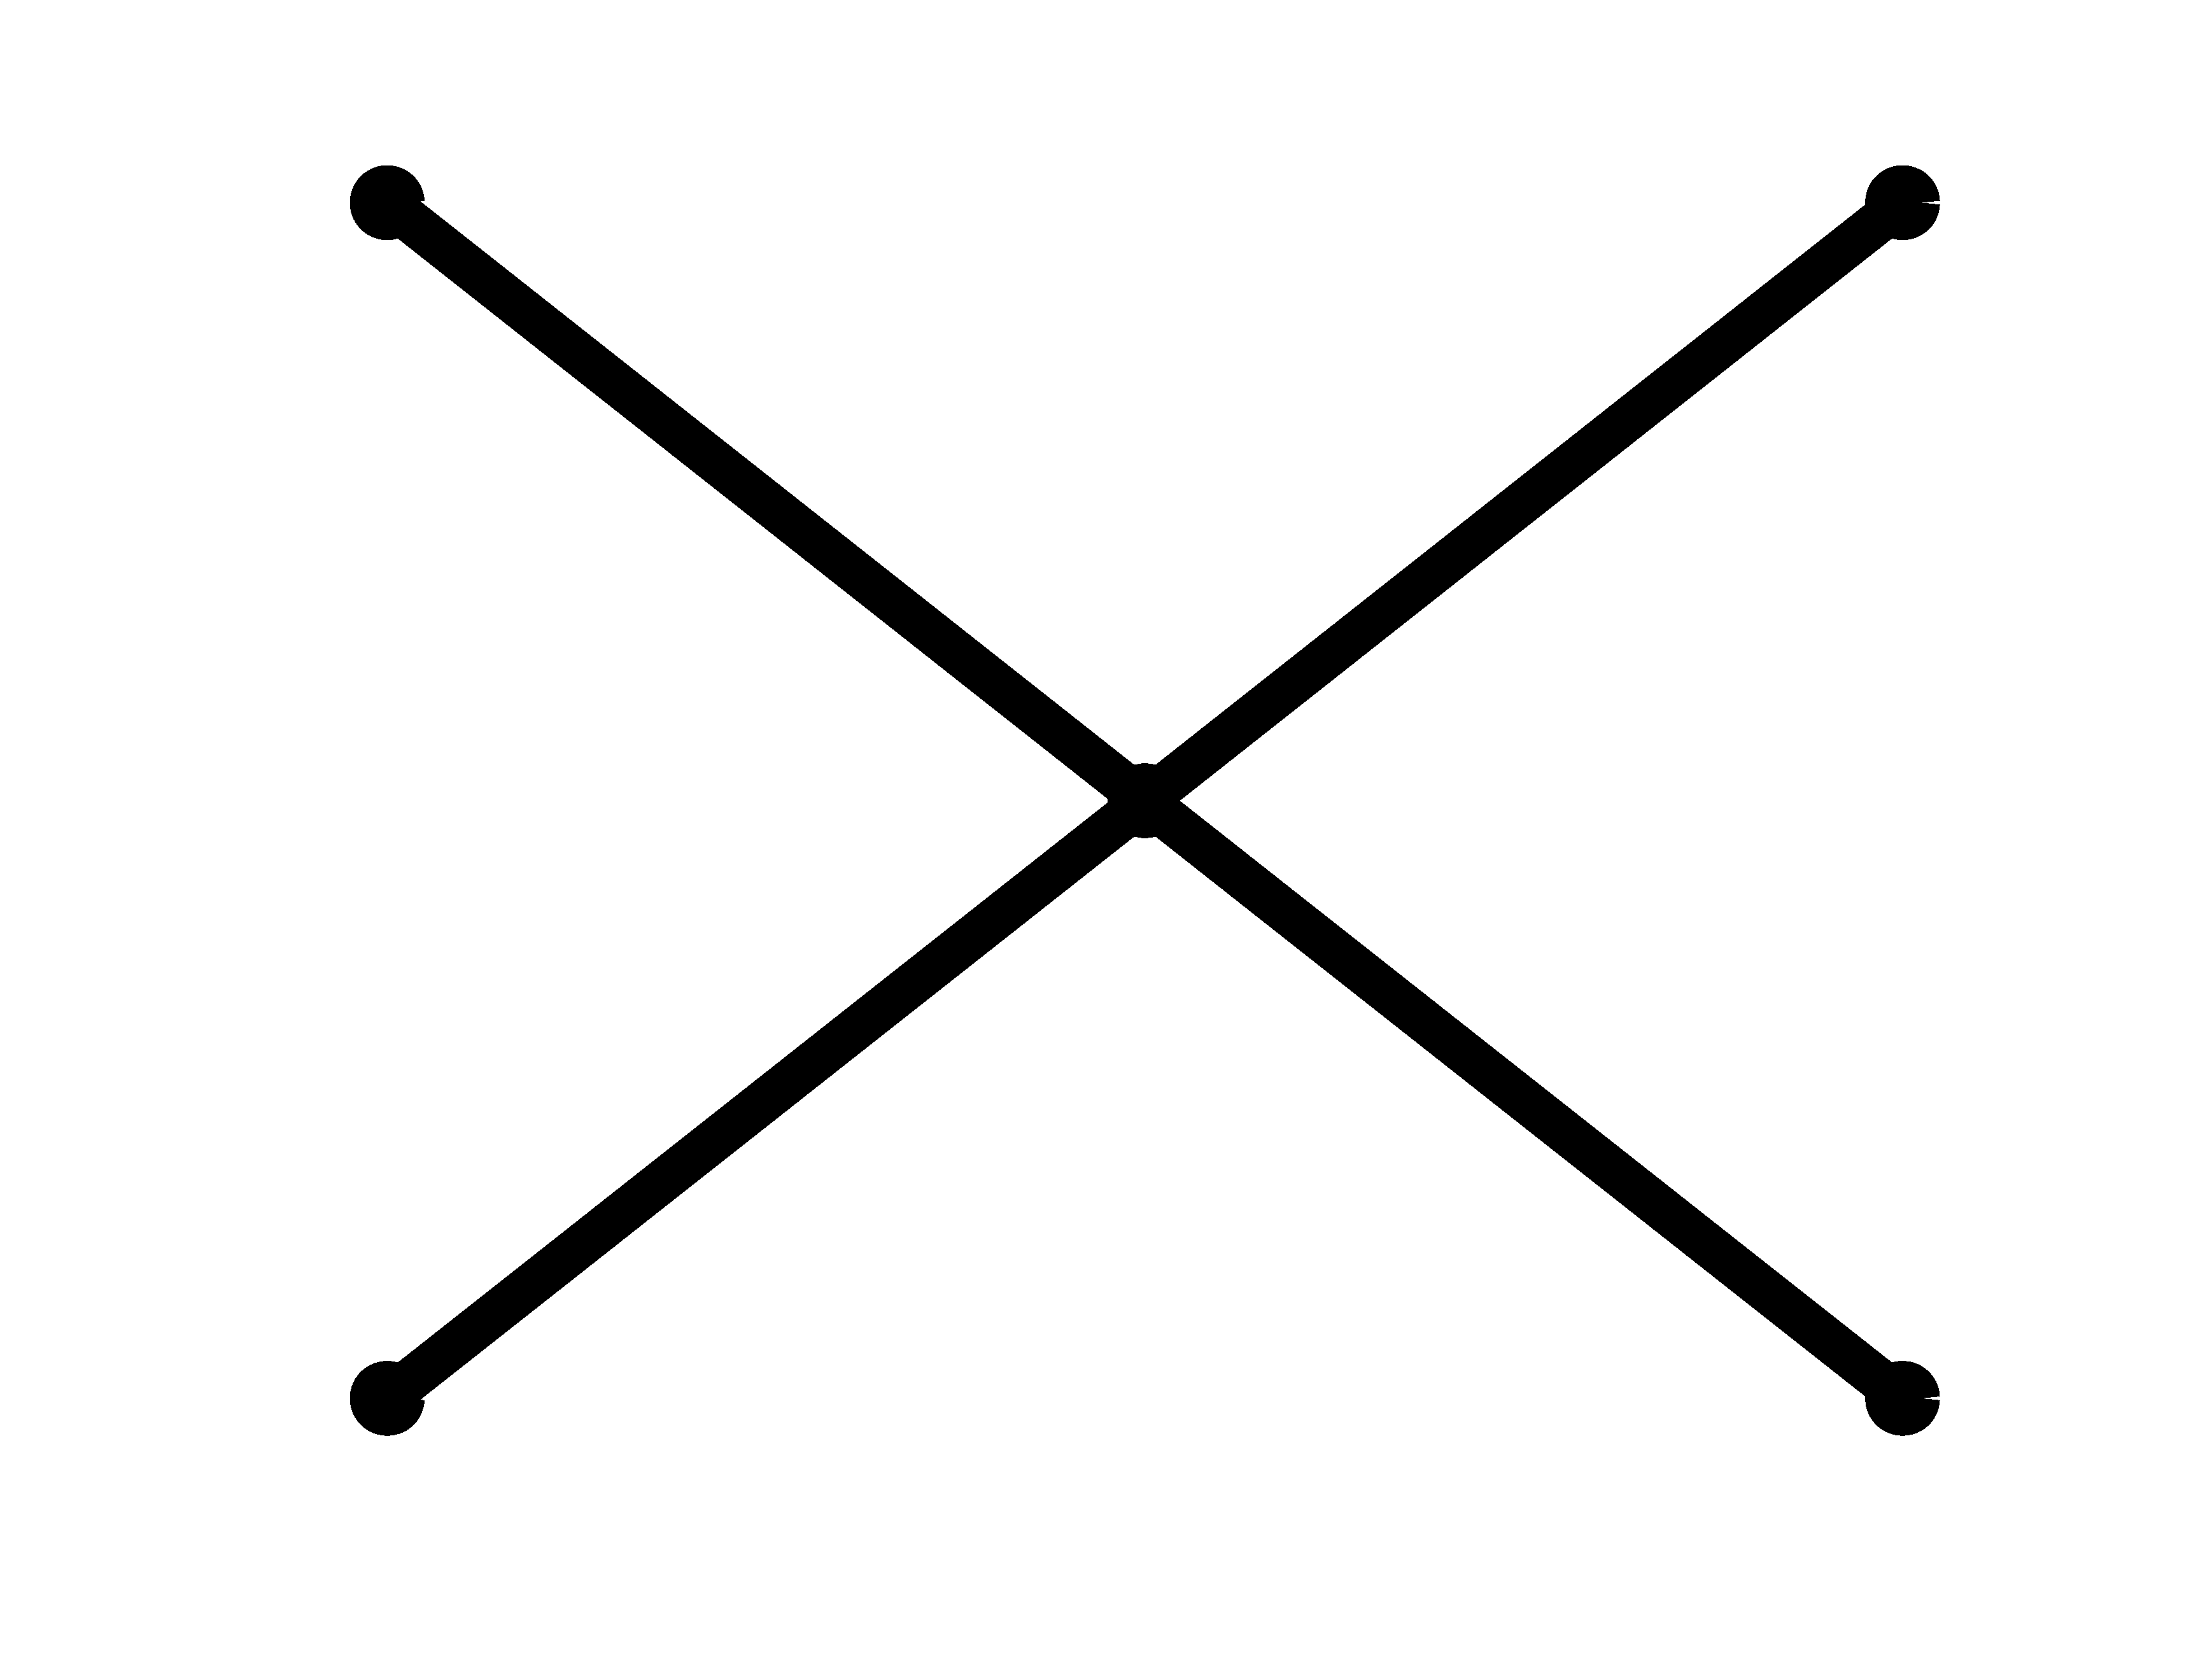
\epsfig{file =
            ../Figures/Motif-Star4.eps, clip=, width=1cm, height=1cm}
        \end{tabular}   
      \end{tabular}  } 
  \end{tabular}
  &
  \begin{tabular}{c}
    \hspace{-1cm}
    \epsfig{file=
      /RECHERCHE/RESEAUX/Motifs/FIGURES/MotifStar4-Recouv3.eps,
      clip=, width=13cm, height=17cm}
  \end{tabular}
\end{tabular}

%\paragraph{Variance.} The formula of the variance follows:
  
%%%%%%%%%%%%%%%%%%%%%%%%%%%%%%%%%%%%%%%%%%%%%%%%%%%%%%%%%%%%%%%%%%%%%
%%%%%%%%%%%%%%%%%%%%%%%%%%%%%%%%%%%%%%%%%%%%%%%%%%%%%%%%%%%%%%%%%%%%%
\newpage
\chapter{Approximate Distribution of the Count}
%%%%%%%%%%%%%%%%%%%%%%%%%%%%%%%%%%%%%%%%%%%%%%%%%%%%%%%%%%%%%%%%%%%%%
%%%%%%%%%%%%%%%%%%%%%%%%%%%%%%%%%%%%%%%%%%%%%%%%%%%%%%%%%%%%%%%%%%%%%

%%%%%%%%%%%%%%%%%%%%%%%%%%%%%%%%%%%%%%%%%%%%%%%%%%%%%%%%%%%%%%%%%%%%%
\bigskip
\section{Calculating the occurrence probability}
%%%%%%%%%%%%%%%%%%%%%%%%%%%%%%%%%%%%%%%%%%%%%%%%%%%%%%%%%%%%%%%%%%%%%

The occurrence probability \emphase{$\mum$} is the central quantity of
this approach. It depends on the random graph model.

\paragraph{Erd�s-Renyi:}
$$
\mum = \prod_{1 \leq u<v \leq k} \pi^{m_{uv}}.
$$

\paragraph{Degree distribution fitting:} Suppose that $D$ has a
distribution proportional to the empirical degree distribution and
denote ${m_{u+}}$ the number of edges of node $u$ in motif $\mbf$,
$$
\mum \propto \prod_{u=1}^k \Esp\left(K^{m_{u+}} \right).
$$

\paragraph{ERMG:}
$$
\mum   =   \sum_{c_1=1}^{Q} \hdots \sum_{c_k=1}^{Q}
\alpha_{c_1}\hdots \alpha_{c_k} \prod_{1 \leq u<v \leq k}
\pi_{c_u,c_v}^{m_{uv}}.
$$

%%%%%%%%%%%%%%%%%%%%%%%%%%%%%%%%%%%%%%%%%%%%%%%%%%%%%%%%%%%%%%%%%%%%%
\newpage
\section{Compound Poisson Approximation for the Count $\Nm$}
%%%%%%%%%%%%%%%%%%%%%%%%%%%%%%%%%%%%%%%%%%%%%%%%%%%%%%%%%%%%%%%%%%%%%

% \paragraph{Gaussian approximation.}
% $
% \Nm \approx \Ncal\left(\Esp[\Nm], \Var[\Nm]\right).
% $

% \paragraph{Poisson approximation.} If $\Var[\Nm] \simeq \Esp[\Nm]$:
% $
% \Nm \approx \Pcal\left(\Esp[\Nm]\right).
% $

\paragraph{Compound Poisson distribution.} All network motifs can overlap (and
constitute super-motifs) so they tend to \emphase{occur in clumps}.
The compound Poisson distribution states that 
\begin{itemize}
\item \vspace{-0.5cm} the number of clumps $C(\mbf)$ has a Poisson
  distribution $\Pcal(\lambda)$;
\item \vspace{-0.5cm} the clump sizes $V_1, ..., V_{C(\mbf)}$ are i.i.d.
\end{itemize}
The count $\Nm$ is the sum of the clump sizes: $\Nm = \sum_c V_c$.

\bigskip\bigskip
\paragraph{Geometric Poisson approximation.} An analogy with
\emphase{sequence motifs} (\refer{RRS05}) suggests that the
clump size has a geometric distribution, $\Gcal(1-a)$ where $a$ is the
\emphase{overlapping probability of the motif}. 

Parameters $\lambda$ and $a$ are related two the first two moments:
$$
a = \frac{\Var\Nm - \Esp\Nm}{\Var\Nm + \Esp\Nm}, \qquad
\lambda = (1-a) \Esp\Nm.
$$

%%%%%%%%%%%%%%%%%%%%%%%%%%%%%%%%%%%%%%%%%%%%%%%%%%%%%%%%%%%%%%%%%%%%%
\newpage
\section{Simulation study}
%%%%%%%%%%%%%%%%%%%%%%%%%%%%%%%%%%%%%%%%%%%%%%%%%%%%%%%%%%%%%%%%%%%%%

\subsection{Simulation design}

\paragraph{Aim:} Compare the Gaussian, Poisson and Geometric-Poisson
approximations for the motif count distribution.

\hspace{-2.2cm}
\begin{tabular}{cc}
  \begin{tabular}{p{12cm}}
    \paragraph{Random graph model:} ERMG with 2 groups.
    \\ \\
    \paragraph{4 motifs:}  \\
    %$$
    \begin{tabular}{cccc}
      $\mathsf{V}$ & triangle & 4-star & square \\
%       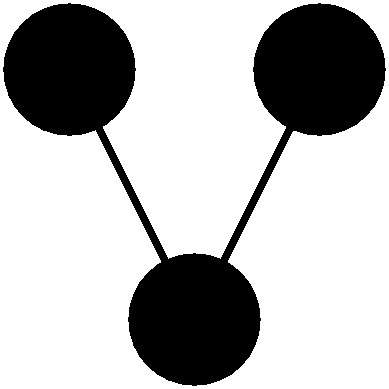
\includegraphics[height=1cm]{../figures/Vmotif.eps} & 
%       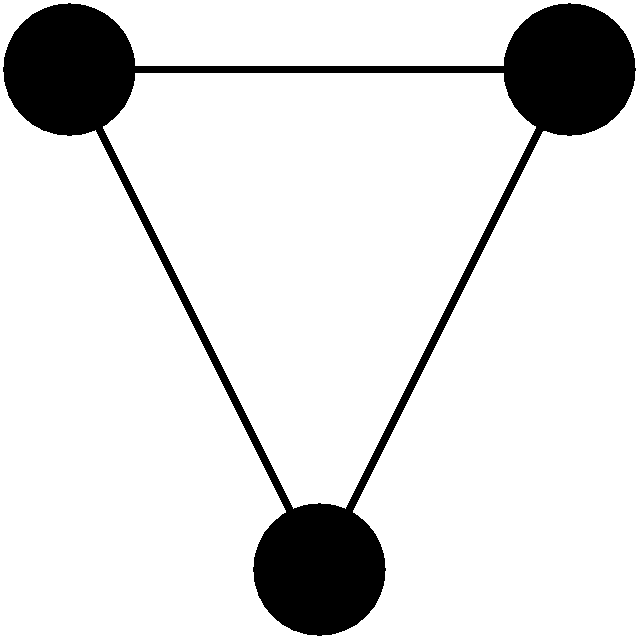
\includegraphics[height=1cm]{../figures/nablamotif.eps} & 
%       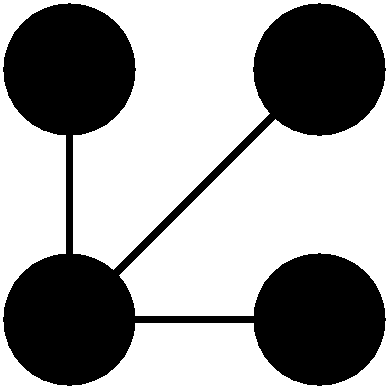
\includegraphics[height=1cm]{../figures/starmotif.eps}  & 
%       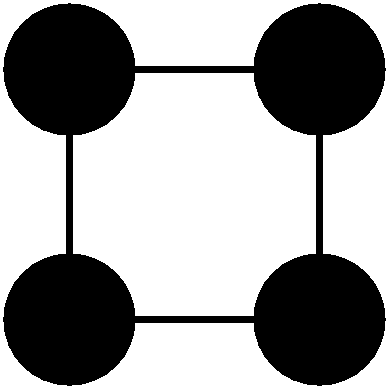
\includegraphics[height=1cm]{../figures/squaremotif.eps}\\
      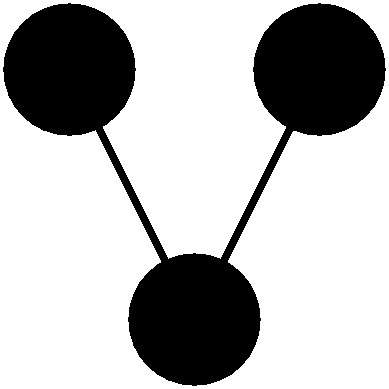
\epsfig{file = ../figures/Vmotif.eps, width=2cm, clip=} & 
      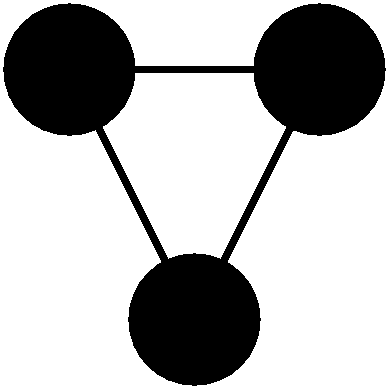
\epsfig{file = ../figures/trianglemotif.eps, width=2cm, clip=} & 
      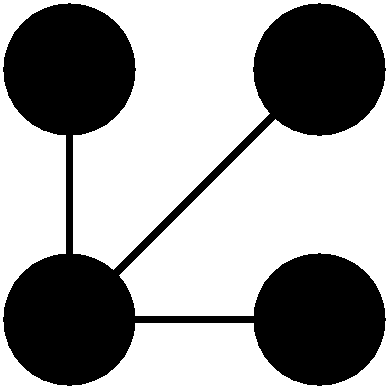
\epsfig{file = ../figures/starmotif.eps, width=2cm, clip=}  & 
      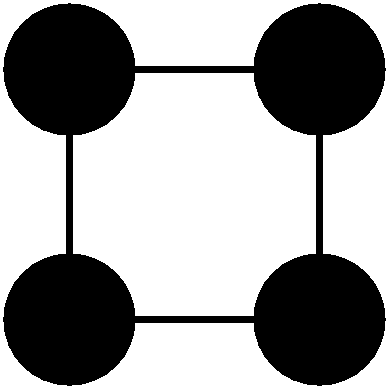
\epsfig{file = ../figures/squaremotif.eps, width=2cm, clip=}
    \end{tabular}
    %$$
  \end{tabular}
  &
  \begin{tabular}{p{12cm}}
    \paragraph{Simulation design:}
    \begin{itemize}
    \item \vspace{-0.5cm} number of vertices $n=20,200$
    \item \vspace{-0.5cm} mean connectivity $\bar{\pi}=1/n,2/n$ 
    \item \vspace{-0.5cm} within/between group connectivity
      $\gamma=0.1,0.5,0.9$ 
    \item \vspace{-0.5cm} proportion of the groups $\alpha=0.1,0.9$
    \end{itemize}
  \end{tabular}
\end{tabular}

\paragraph{Expected frequency:}
We cover a large range for $\Esp N(\mbf)$ (from 0.07 to 1075.5).

\hspace{-1.75cm}
\begin{tabular}{cl}
  \paragraph{Criterion:} & $D =$ total variation distance, \\
  & $\widehat{F} = $ actual level of the 99\% theoretical quantile.
\end{tabular}

%%%%%%%%%%%%%%%%%%%%%%%%%%%%%%%%%%%%%%%%%%%%%%%%%%%%%%%%%%%%%%%%%%%%%
\newpage
\subsection{Expectedly frequent motif count distribution}

\hspace{-2.2cm}
\begin{tabular}{cc}
  \multicolumn{2}{c}{Gaussian ($G = $ \textcolor{red}{--}), Poisson (--) and
    Geometric-Poisson ($GP = $ \textcolor{green}{--})} \\
    Histogram & PP-plot \\
    \epsfig{file = ../figures/hist_200_0.005_0.5_0.1_V.eps,
    width=12cm, clip=} 
    &
    \epsfig{file = ../figures/PPPlot_200_0.005_0.5_0.1_V.eps,
    width=12cm, clip=}  
\end{tabular} \\
\hspace*{-1cm}
\begin{tabular}{cc}
  {\small simulation parameters} &  motif $\Vsf$ \\
  {\small
    \begin{tabular}{c|c|c|c}
      $n$ & $\overline{\pi}$ & $\alpha$ (\%)& $\gamma$ (\%)\\ \hline
      200     & 0.5   & 10    & 10   \\
      200     & 0.5   & 10    & 90   \\
      200     & 0.5   & 50    & 10   \\
      200     & 0.5   & 50    & 50   \\
      200     & 0.5   & 50    & 90  \\
    \end{tabular} 
    } 
  &
  {\small
    \begin{tabular}{c|c|c|c|c|c|c|c}
      $\Esp$ & $\mathbb{V}$ & $\lambda$ & $\frac{1}{1-a}$  & $D_G$ & $D_{GP}$ &
      $\hat{F}_G$ & \emphase{$\hat{F}_{GP}$} \\ \hline
      159.5   & 2034.0        & 23.1 & 6.66   & 20.4 & 19.7 & 2.5 & \emphase{1.6} \\
      104.9   & 590.5         & 31.6 & 3.33   & 15.2 & 14 & 1.9 & \emphase{1.2}\\
      98.5    & 484.0         & 33.3 & 2.27   & 13.1 & 12.6 & 1.1 & \emphase{0.7}\\
      98.5    & 484.0         & 33.2 & 2.27   & 14.3 & 13.2 & 1.6 & \emphase{1.1}\\
      98.5    & 488.4         & 33.1 & 2.27   & 14.5 & 14.8 & 2.5 & \emphase{0.9}\\
    \end{tabular}
    }
  \\
\end{tabular}

%%%%%%%%%%%%%%%%%%%%%%%%%%%%%%%%%%%%%%%%%%%%%%%%%%%%%%%%%%%%%%%%%%%%%
\newpage
\subsection{Expectedly rare motif count distribution}

\hspace{-2.2cm}
\begin{tabular}{cc}
  \multicolumn{2}{c}{Gaussian ($G = $ \textcolor{red}{--}), Poisson (--) and
    Geometric-Poisson ($GP = $ \textcolor{green}{--})} \\
    Histogram & PP-plot \\
    \epsfig{file = ../figures/hist_200_0.01_0.1_0.1_C.eps, 
    width=12cm, clip=} 
    &
    \epsfig{file = ../figures/PPPlot_200_0.01_0.1_0.1_C.eps,
    width=12cm, clip=}  
\end{tabular} \\
\hspace*{-1cm}
\begin{tabular}{cc}
  {\small simulation parameters} &  motif $\square$ \\
  {\small
    \begin{tabular}{c|c|c|c}
      $n$ & $\overline{\pi}$ & $\alpha$ (\%)& $\gamma$ (\%)\\ \hline
      200     & 0.5   & 10    & 10   \\
      200     & 0.5   & 10    & 90   \\
      200     & 0.5   & 50    & 10   \\
      200     & 0.5   & 50    & 50   \\
      200     & 0.5   & 50    & 90  \\
    \end{tabular} 
    } 
  &
  {\small
    \begin{tabular}{c|c|c|c|c|c|c|c}
      $\Esp$ & $\mathbb{V}$ & $\lambda$ & $\frac{1}{1-a}$  & $D_G$ & $D_{GP}$ &
      $\hat{F}_G$ & \emphase{$\hat{F}_{GP}$} \\ \hline
      7.31&21.72&3.68& 2 &11.8&5.4&3.2&\emphase{0.9}\\
      2.57&3.42&2.21 & 1.16 &9.3&2.7&3.6&\emphase{0.5}\\
      2.74&3.69&2.33 & 1.17 &12.3&3.6&4.7&\emphase{1.2}\\
      1.94&2.40&1.74 & 1.11  &11.3&2.0&3.2&\emphase{1.6}\\
      2.74&3.72&2.32 & 1.17 &10.8&4.5&3.7&\emphase{0.7}\\
    \end{tabular}
    }
  \\
\end{tabular}

%%%%%%%%%%%%%%%%%%%%%%%%%%%%%%%%%%%%%%%%%%%%%%%%%%%%%%%%%%%%%%%%%%%%%
\newpage
\section{Conclusions for the simulation study}

\begin{itemize}
\item Correct analytical expressions for $\Esp N$ and
  $\Var N$ (simulations not shown).
\item Bad fit of the Poisson approximation.
\item \emphase{Geometric-Poisson outperforms Gaussian}
  for both criteria in all cases, especially for ``rare'' motifs.
\item \emphase{Underestimation of the 99\% quantile}
  with the Gaussian approximation, \\
  {\bf{$\rightarrow$}} false positive results.
\item \emphase{High total variation distance} for both
  approximations in some cases, especially for frequent and highly
  self overlapping motifs.
\item The clumps size distribution is probably \emphase{not geometric}
  $\ldots$
\end{itemize}

%%%%%%%%%%%%%%%%%%%%%%%%%%%%%%%%%%%%%%%%%%%%%%%%%%%%%%%%%%%%%%%%%%%%%
%%%%%%%%%%%%%%%%%%%%%%%%%%%%%%%%%%%%%%%%%%%%%%%%%%%%%%%%%%%%%%%%%%%%%
\newpage
\chapter{Application to the {\it H. pylori} PPI network}
%%%%%%%%%%%%%%%%%%%%%%%%%%%%%%%%%%%%%%%%%%%%%%%%%%%%%%%%%%%%%%%%%%%%%
%%%%%%%%%%%%%%%%%%%%%%%%%%%%%%%%%%%%%%%%%%%%%%%%%%%%%%%%%%%%%%%%%%%%%

Protein-protein interaction network: 706 proteins (nodes) and 1420
interactions (edges).

\hspace{-2cm}
\begin{tabular}{cc}
  \begin{tabular}{p{12cm}}
    \subsection{Fit of ERMG} \\
    \begin{itemize}
    \item \vspace{-0.5cm} ERMG was fitted to the network and
      \emphase{4 groups} of connectivity were selected using a model
      selection criterion (ICL).
    \item \vspace{-0.5cm} Goodness-of-fit for the degree distribution
      assessed by PP-plot (right).
    \end{itemize}
  \end{tabular}
  &
  \begin{tabular}{c}
    \epsfig{file = ../figures/hist-deg-HPylo.eps, width=10cm, clip=}   
  \end{tabular}
\end{tabular}

%%%%%%%%%%%%%%%%%%%%%%%%%%%%%%%%%%%%%%%%%%%%%%%%%%%%%%%%%%%%%%%%%%%%%
\newpage
\subsection{Significance of motifs of size 3 and 4}

2 motifs appear to be unexpectedly frequent.
$$
\begin{tabular}{crrrrrr}
 Motif & $N_{\obs}(\mbf)$ & $\Esp_{\ERMG}(N)$ & $\sigma_{\ERMG}(N)$ &
 $\lambda$ & $1/(1-a)$ & $p$-value  \\

 \hline
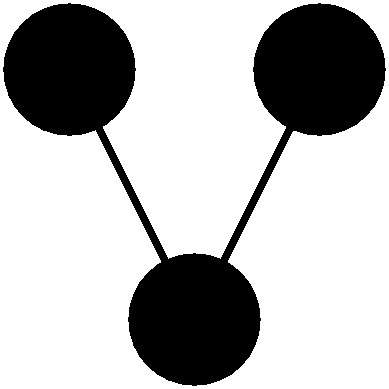
\epsfig{file = ../figures/Vmotif.eps, width=1cm, clip=} & 14\,113 & 13\,118 & 2\,599 & 25.5 & 514.9 & 3.36$\,10^{-1}$ \\
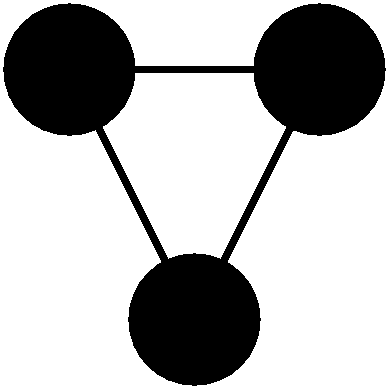
\epsfig{file = ../figures/trianglemotif.eps, width=1cm, clip=} & 75 & 64.4 & 20 & 10.4 & 6.2 & 2.87$\,10^{-1}$ \\
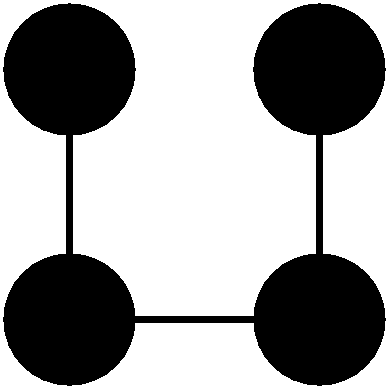
\epsfig{file = ../figures/chainmotif.eps, width=1cm, clip=} & 98\,697 & 90\,059 & 26\,064 & 11.9 & 7\,543.2 & 3.46$\,10^{-1}$ \\
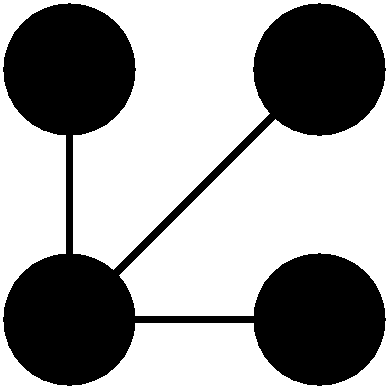
\epsfig{file = ../figures/starmotif.eps, width=1cm, clip=} & 112\,490 & 89\,372 & 26\,423 & 11.4 & 7\,812.0 & 1.85$\,10^{-1}$ \\
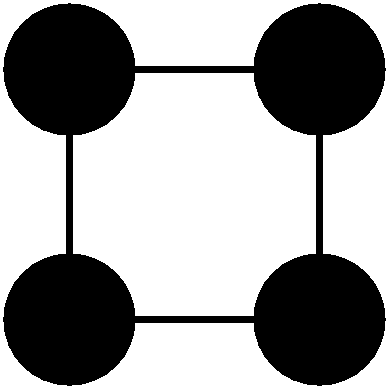
\epsfig{file = ../figures/squaremotif.eps, width=1cm, clip=} & 1\,058 & 492 & 202 & 5.9 & 82.9 & \emphase{9.34$\,10^{-3}$} \\
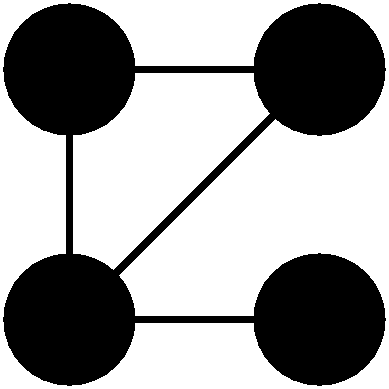
\epsfig{file = ../figures/whisker.eps, width=1cm, clip=} & 3\,535 & 2\,756 & 1\,087 & 6.4 & 428.7 & 2.22$\,10^{-1}$ \\
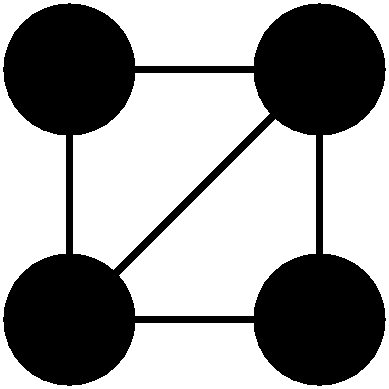
\epsfig{file = ../figures/halfclique.eps, width=1cm, clip=} & 79 &
 33.2 & 19.5 & 2.9 & 11.5 & \emphase{2.56$\,10^{-2}$} \\
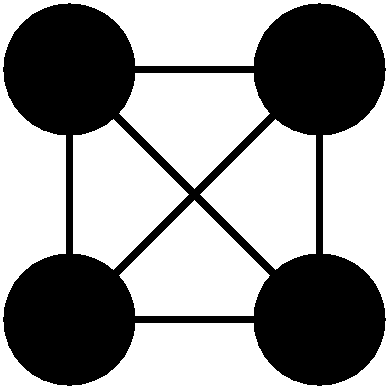
\epsfig{file = ../figures/clique.eps, width=1cm, clip=} & 0 & 0.165 & 0.432 & 0.1 & 1.1 & 1.00 \\
\end{tabular}
$$
\paragraph{Mean clump size.} $\Esp V = 1/(1-a)$.

%%%%%%%%%%%%%%%%%%%%%%%%%%%%%%%%%%%%%%%%%%%%%%%%%%%%%%%%%%%%%%%%%%%%%
\newpage
\section{Comparison with the Mfinder software}
%%%%%%%%%%%%%%%%%%%%%%%%%%%%%%%%%%%%%%%%%%%%%%%%%%%%%%%%%%%%%%%%%%%%%

\bigskip
\centerline{{\tt Mfinder: www.weizmann.ac.il/mcb/UriAlon/}}

\bigskip
\hspace{-2cm}
\begin{tabular}{ll}
  \begin{tabular}{p{10cm}}
    \subsection{Motifs of size 3 and 4:} \\
    \\
    \emphase{All motifs are significantly} over- or
    under-represented...\\
    \\
    All empirical $p$-values are equal either to 0 or 1 (not shown). \\
    \\
    Simular results with 1000 simulated graphs. \\
    \\
  \end{tabular}
  &
  \hspace{-1.5cm}
  \begin{tabular}{c}
    {\small
      \begin{tabular}{c|r|rr|rrr|c} 
        Motif & $N_{\text{obs}}$ &
        $\overline{N}_{100}$&$\overline{\sigma }_{100}$&Z-score &
        $\Ncal$ $$p$$-value \\
        \hline
        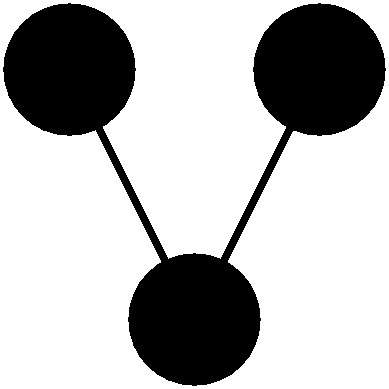
\epsfig{file = ../figures/Vmotif.eps, width=1cm, clip=}     &  13\,888 
        & {13\,648} & {51.8} & \emphase{4.63} & {1.82\,10${^{-6}}$}    \\
        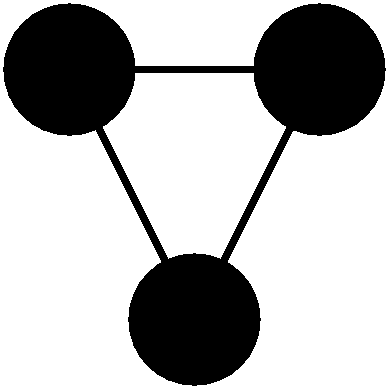
\epsfig{file = ../figures/trianglemotif.eps, width=1cm, clip=}   &  75    
        & {155}   & {17.3} & \emphase{-4.63}& {1.82\,10${^{-6}}$}     \\
        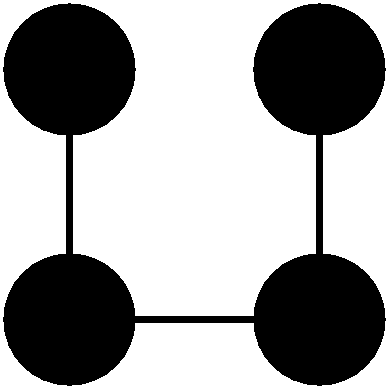
\epsfig{file = ../figures/chainmotif.eps, width=1cm, clip=} &  87\,869 
        & {112\,532} & {1\,957} & \emphase{-12.60}& {1.05\,10${^{-36}}$}  \\
        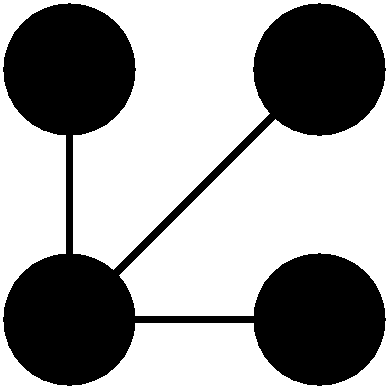
\epsfig{file = ../figures/starmotif.eps, width=1cm, clip=}  &  109\,113
        & {103\,186} & {1\,084} & \emphase{5.47}& {2.27\,10${^{-8}}$}     \\
        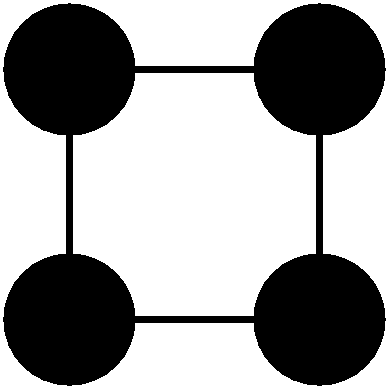
\epsfig{file = ../figures/squaremotif.eps, width=1cm, clip=}&  979   
        & {796} & {64.7} & \emphase{2.84}& {2.25\,10${^{-3}}$}    \\
        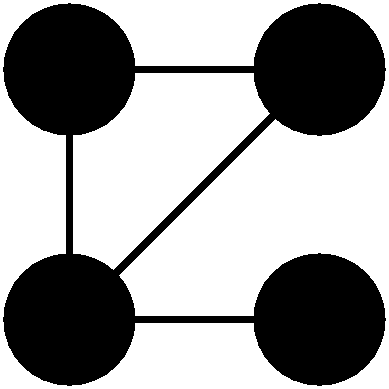
\epsfig{file = ../figures/whisker.eps, width=1cm, clip=}      &  3\,219  
        & {8\,734} & {945} & \emphase{-5.84}& {2.61\,10${^{-9}}$}   \\
        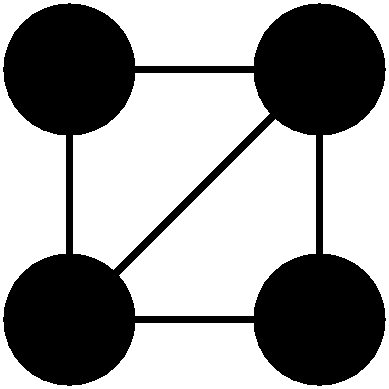
\epsfig{file = ../figures/halfclique.eps, width=1cm, clip=} &  79    
        & {273} & {66.7}& \emphase{-2.90}& {1.85\,10${^{-3}}$}    \\
        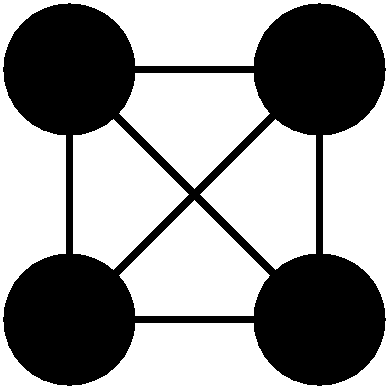
\epsfig{file = ../figures/clique.eps, width=1cm, clip=}     &  0     
        & {6.2} & {3.7} & \emphase{-1.70}& {4.45\,10${^{-2}}$}       
      \end{tabular}
      }
  \end{tabular}
\end{tabular}

\bigskip
\paragraph{Direct comparison can not be made} since MFinder considers
'induced' motifs, e.g. pure 'V', pure square, etc.

%%%%%%%%%%%%%%%%%%%%%%%%%%%%%%%%%%%%%%%%%%%%%%%%%%%%%%%%%%%%%%%%%%%%%
\newpage
\subsection{About the Mfinder 'model'}

\bigskip
\paragraph{The model is not explicit.} The edge swapping algorithm
aims at sampling (uniformly?) among all the graphs with same degree
sequence. The independence of the simulations relies on a
\emphase{large number of swaps}.

\bigskip
\paragraph{The edge swapping algorithm} does not really affect \emphase{strong
  network structure}, such as hubs (resulting in small estimated
variance for star motifs). \\
The variabilty of the 'V' count is only due to the variability of
number of triangles.

\bigskip
\paragraph{What is the fit} of a model declaring that \emphase{all
  motifs} are significant?

%%%%%%%%%%%%%%%%%%%%%%%%%%%%%%%%%%%%%%%%%%%%%%%%%%%%%%%%%%%%%%%%%%%%%
\bigskip\bigskip
\subsection{New simulations}

\paragraph{Exact degree fitting (EDF) model.} We sampled without
replacement in the observed degree distribution $\widehat{F}$ (similar
to edge swapping in MFinder).

\paragraph{Motif.} For each simulated graphs we counted the number of
occurrences of each motif (with our definition). 

%%%%%%%%%%%%%%%%%%%%%%%%%%%%%%%%%%%%%%%%%%%%%%%%%%%%%%%%%%%%%%%%%%%%%
\newpage
\subsection{Results for {\sl H. pylori.} PPI network}
$$
\begin{tabular}{cc}
  \begin{tabular}{p{9cm}}
    \paragraph{Comparison ERMG / EDF.}\\
    \\ \\
    Degree distribution fitting is a very strong constraint. \\
    \\ \\
    The number of occurrences of \emphase{star-like motifs} ('V', hubs,
    {\it etc.})  is \emphase{completely fixed} in the EDF model.
    \\ \\
  \end{tabular}
  &
  \begin{tabular}{c}
    \hspace{-1cm}
    \begin{tabular}{c|rr|rr}
      & \multicolumn{2}{c|}{$\overline{N}$} & \multicolumn{2}{c}{$\sigma(N)$} \\
      Motif & ERMG & EDF & ERMG & EDF \\
      \hline
      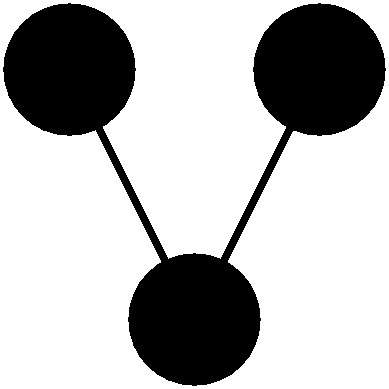
\epsfig{file = ../figures/Vmotif.eps, width=1cm, clip=}         & 13 118  & 14 113  & 2 599   & \emphase{0} \\
      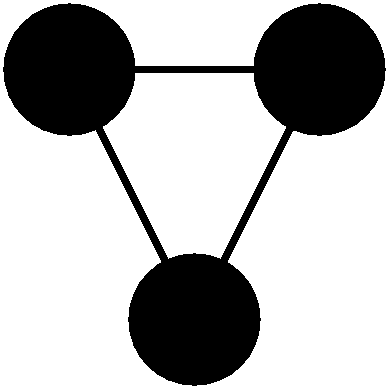
\epsfig{file = ../figures/trianglemotif.eps, width=1cm, clip=}       & 64      & 53      & 20      & 8       \\
      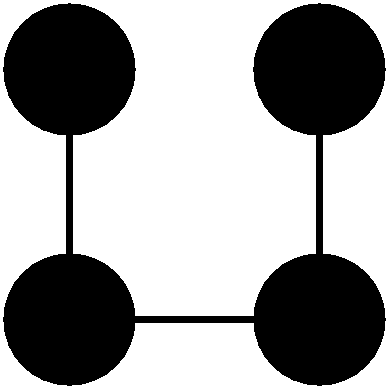
\epsfig{file = ../figures/chainmotif.eps, width=1cm, clip=}     & 90 059  & 84 106  & 26 064  & 3 283   \\
      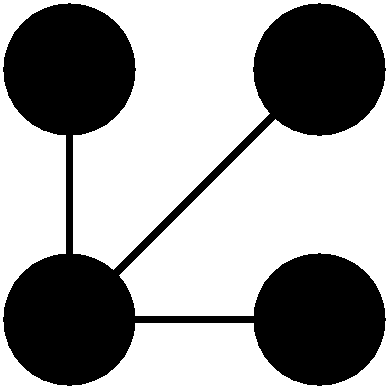
\epsfig{file = ../figures/starmotif.eps, width=1cm, clip=}      & 89 372  & 112 490 & 26 423  & \emphase{0} \\
      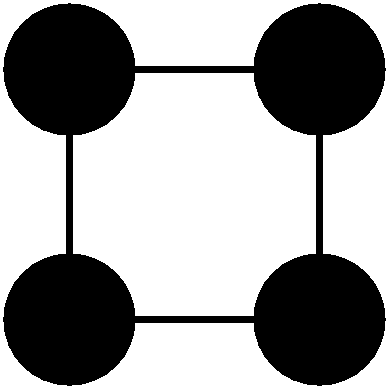
\epsfig{file = ../figures/squaremotif.eps, width=1cm, clip=}    & 492     & 285     & 202     & 27      \\
      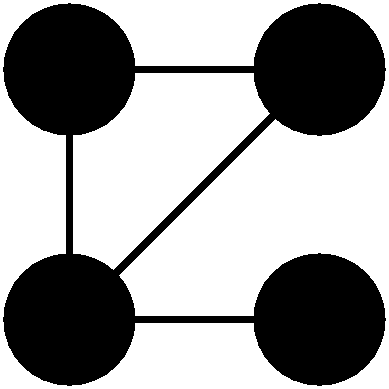
\epsfig{file = ../figures/whisker.eps, width=1cm, clip=}          & 2 756   & 2 412   & 1 087   & 447     \\
      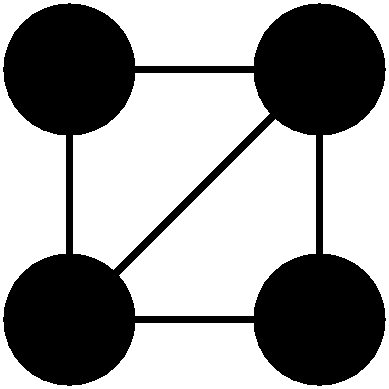
\epsfig{file = ../figures/halfclique.eps, width=1cm, clip=}     & 33      & 22      & 20      & 10      \\
      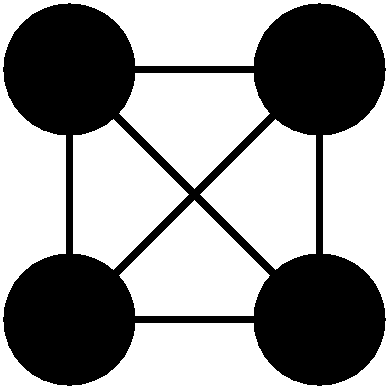
\epsfig{file = ../figures/clique.eps, width=1cm, clip=}        & 0.2     &  0.1     &  0.4     &   0.3     \\
    \end{tabular}
  \end{tabular}
\end{tabular}
$$

%%%%%%%%%%%%%%%%%%%%%%%%%%%%%%%%%%%%%%%%%%%%%%%%%%%%%%%%%%%%%%%%%%%%%
\newpage
\section{Conclusions and Future Works}
%%%%%%%%%%%%%%%%%%%%%%%%%%%%%%%%%%%%%%%%%%%%%%%%%%%%%%%%%%%%%%%%%%%%%

\begin{itemize}
\item \vspace{-0.5cm} We propose a general method to \emphase{assess
    the exceptionality of network motifs}.
\item \vspace{-0.5cm} The formula of the moments are valid for a
  \emphase{large class} of random graphs.
\item \vspace{-0.5cm} The \emphase{geometric Poisson approximation
    performs well} (better than Gaussian and Poisson) on simulated
  data.
\end{itemize}

%%%%%%%%%%%%%%%%%%%%%%%%%%%%%%%%%%%%%%%%%%%%%%%%%%%%%%%%%%%%%%%%%%%%%
\subsection{Open questions}

\begin{itemize}
\item \vspace{-0.5cm} Insights about the \emphase{distribution of the
    clump size} (other than geometric) would improve the compound
  Poisson approximation. 
\item \vspace{-0.5cm} \emphase{A colored motif} is a connected subset
  set of colored. Such motifs can describe protein complexes, the
  proteins being classified into functions.  \\
  \centerline{$\Rightarrow$ How to assess their exceptionality?}
\item \vspace{-0.5cm} \emphase{What is a relevant random graph model}
  for motif detection. \\
  \centerline{$\Rightarrow$ What properties should it satisfy?}
\end{itemize}
  
% %%%%%%%%%%%%%%%%%%%%%%%%%%%%%%%%%%%%%%%%%%%%%%%%%%%%%%%%%%%%%%%%%%%%%
% \newpage
% \subsection{Model comparison}

% \paragraph{Mixture model for random graphs (ERMG).} Described above, fitted
% to the observed graph.

% \paragraph{Exact degree fitting (EDF).} Sampling without replacement in the
% observed degree distribution $\widehat{F}$ (similar to edge swapping
% in MFinder).

% \paragraph{Approximate degree fitting (ADFa).} Sampling with replacement in
% $\widehat{F}$.

% \paragraph{Approximate degree fiting (ADFb).} Labeling each edge with a 'mean
% degree' $D_i$ sampled with replacement in $\widehat{F}$, then
% generating each edge with probability
% $$
% \Pr\{i \sim j | D_i, D_j\} = \kappa D_i D_j.
% $$
% (Depending on $\kappa$, this probability may exceed one!).

% % \paragraph{Approximate degree fiting (ADFb').} Dame as (B) with smaller
% % coefficient to make all $\kappa D_i D_j \leq 1$.


% %%%%%%%%%%%%%%%%%%%%%%%%%%%%%%%%%%%%%%%%%%%%%%%%%%%%%%%%%%%%%%%%%%%%%
% \newpage
% \subsection{Results for {\sl H. pylori.}}
% $$
% {
% \begin{tabular}{c|rrrr|rrrr}
%   & \multicolumn{4}{c|}{Mean $\Esp N$} & \multicolumn{4}{c}{Standard
%   deviation $\sqrt{\Var N}$} \\
%   Motif & ERMG & EDF & ADFa & ADFb & ERMG & EDF & ADFa & ADFb \\
%   \hline
%   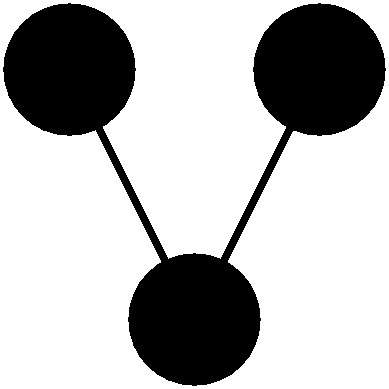
\epsfig{file = ../figures/Vmotif.eps, width=1cm, clip=}      & 13 118 & 14 113 & 14 151 & 15 444 & 2 599 & 0 & 2 510 & 4 200 \\
%   \epsfig{file = ../figures/triangle.eps, width=1cm, clip=}    & 64 & 53 & 55 & 249 & 20 & 8 & 19 & 132 \\
%   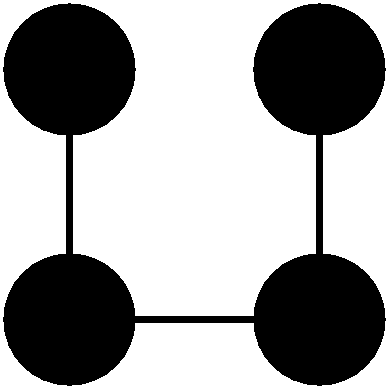
\epsfig{file = ../figures/chainmotif.eps, width=1cm, clip=}  & 90 059 & 84 106 & 85 874 & 176 040 & 26 064 & 3 283 & 23 397 & 78 751 \\
%   \epsfig{file = ../figures/starmotif.eps, width=1cm, clip=}   & 89 372 & 112 490 & 112 880 & 126 510 & 26 423 & 0 & 36 104 & 58 096 \\
%   \epsfig{file = ../figures/squaremotif.eps, width=1cm, clip=} & 492 & 285 & 303 & 2 128 & 202 & 27 & 132 & 1 545 \\
%   \epsfig{file = ../figures/whisk.eps, width=1cm, clip=}      & 2 756 & 2 412 & 2 547 & 18 353 & 1 087 & 447 & 1 208 & 13 492 \\
%   \epsfig{file = ../figures/halfclique.eps, width=1cm, clip=} & 33 & 22 & 25 & 957 & 20 & 10 & 19 & 1 042 \\
%   \epsfig{file = ../figures/clique.eps, width=1cm, clip=} & 0 & 0 & 0
%   & 36 & 0 & 0 & 0 & 56 \\
% \end{tabular}
% }
% $$
% Degree distribution fitting is a very strong constraint. \\
% %\\
% The number of occurrences of \emphase{star-like motifs} ('V', hubs,
% {\it etc.})  are \emphase{completely fixed} in the EDF model.

%%%%%%%%%%%%%%%%%%%%%%%%%%%%%%%%%%%%%%%%%%%%%%%%%%%%%%%%%%%%%%%%%%%%%
\newpage
{\small
  \bibliography{/Biblio/ARC,/Biblio/SSB}
  \bibliographystyle{/Latex/astats}
}

%%%%%%%%%%%%%%%%%%%%%%%%%%%%%%%%%%%%%%%%%%%%%%%%%%%%%%%%%%%%%%%%%%%%%%%%
%%%%%%%%%%%%%%%%%%%%%%%%%%%%%%%%%%%%%%%%%%%%%%%%%%%%%%%%%%%%%%%%%%%%%%%%
%%%%%%%%%%%%%%%%%%%%%%%%%%%%%%%%%%%%%%%%%%%%%%%%%%%%%%%%%%%%%%%%%%%%%%%%
%%%%%%%%%%%%%%%%%%%%%%%%%%%%%%%%%%%%%%%%%%%%%%%%%%%%%%%%%%%%%%%%%%%%%%%%
\end{document}
%%%%%%%%%%%%%%%%%%%%%%%%%%%%%%%%%%%%%%%%%%%%%%%%%%%%%%%%%%%%%%%%%%%%%%%%
%%%%%%%%%%%%%%%%%%%%%%%%%%%%%%%%%%%%%%%%%%%%%%%%%%%%%%%%%%%%%%%%%%%%%%%%
%%%%%%%%%%%%%%%%%%%%%%%%%%%%%%%%%%%%%%%%%%%%%%%%%%%%%%%%%%%%%%%%%%%%%%%%
%%%%%%%%%%%%%%%%%%%%%%%%%%%%%%%%%%%%%%%%%%%%%%%%%%%%%%%%%%%%%%%%%%%%%%%%

